\section{The OAuth Protocol}

\textbf{OAuth} is an open protocol to allow secure API
authorization in a simple and standard message flow from desktop and web
applications. \cite{oauth} \cite{rfc}
It enables \textbf{users} to
authenticate through a \textbf{service provider} and authorize third party applications called
\textbf{OAuth consumers} to access data that is associated with a
\textbf{restricted resource} managed by the
service provider.

\begin{figure}
	\centering
	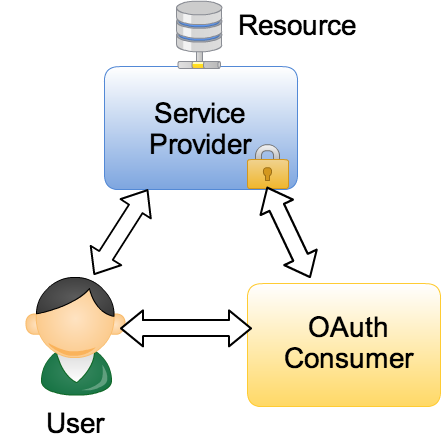
\includegraphics[resolution=200]{../HPI-IP-OAuth/raw/master/OAuth.png}
	\caption{The three parties in OAuth protocol. The user owns the restricted resource and can grant access to it.}
\end{figure}

In order to authenticate an user and enable authorization an
OAuth consumer has to be registered at the service provider
beforehand. Through registration the service provider obtains a
dedicated consumer key \& secret pair that is used for
authenticating the service whenever user access is requested. This
is an significant difference towards the OpenID protocol where
identity provider and relying party don't need to know each other
and the authentification is done decentral. \cite{openid} 

\subsection{OAuth authentication flow}

When a user wants to authenticate a webservice via OAuth the
\textbf{OAuth authentication flow} (commonly referred to as the
OAuth dance) is executed.

The following description is a simplified OAuth description as
details important for securing the authorization flow and protect
it from replay attacks like the \emph{signature method} and
\emph{nonce} are ommitted. The description is first and foremost
meant to provide a general understanding of the OAuth
authentication flow as an full description is beyond the scope of
this paper.

The authentication flow pictured in Fig. \ref{pic:oauth-flow} is started
by the user clicking on a special link on the website of the OAuth consumer.
The consumer uses his consumer key and secret to request an
\textbf{unauthorized OAuth request token} and \textbf{secret} from
the service provider. This OAuth token is used to identify the
authentication context for the user.

After obtaining the request token, the user is redirected from the
consumer to the service provider. Thereby the request token is
appended to the URL. The user is authenticated and can now
authorize the consumer. After the user granted access to the
restricted resource the service provider directs the user's web
agent back to the consumer. A \emph{verifier} is appended to the
callback url.

When the user returns to the consumer the consumer uses request
token and verifier to request an \textbf{access token} and the
associated secret from the service provider. The service provider
exchanges the request token for the access token thereby granting
access to the user's resource(s) as long as the token is valid.


\begin{figure}
	\label{pic:oauth-flow} 
	\centering
	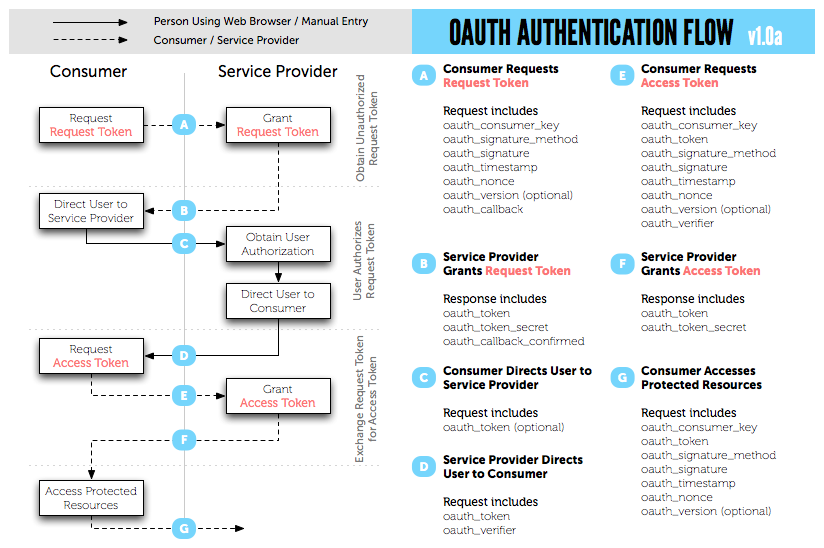
\includegraphics[width=\textwidth]{../oauth_diagram.png}
	\caption{The OAuth authentication flow. \cite{oauth-flow-chart} } 
\end{figure}

%\\source:
%\href{http://dev.twitter.com/pages/auth}{http://dev.twitter.com/pages/auth}
